\section{Factor Graphs}

For problems that include complex relations among many variables it is useful to have an abstract representation of how those	variables interact with each other. So called \emph{factor graphs} are such representations.\newline

In general, a factor graph represents the structure of a function's factorization into smaller functions. \newline If a function $f(X_1, \ldots, X_n)$ can be written as a product $\prod_{j=1}^{m}{f_j(S_j)}$  where the functions $f_j$ have smaller inputs $S_j \subset X$, its factorization 
can be expressed by a factor graph: The graph has two types of nodes: 
\emph{Variable nodes} that correspond to the variables $X_i$ and \emph{factor nodes} corresponding to the functions $f_j$. An edge connects a variable node $X_i$ to a factor node $f_j$ if and only if $X_i$ is part of $f_j$'s input. 
This means the graph is an undirected bipartite graph with the node set $ V = \{X_1, \ldots, X_n\} \cup \{f_1, \ldots, f_n\}$ and edge set $E = \{(X_i, f_j) \; | \; X_i \in S_j\}$. 

In many applications the global function $f$ is a joined probability distribution that can be factorized by using information about independence between the variables. Typical tasks on factor graphs are computing variable assignments that maximize or minimize $f$ or computing marginal distributions if $f$ is a probability distribution. Both of these will be done in Section \ref{BPFS}.

\begin{example}
For random variables $X_1, X_2 \text{ and } X_3$ their joined probability distribution $f$ is defined as $f(x_1, x_2, x_3) := P(X_1 = x_1 \land X_2  = x_2 \land X_3 = x_3)$. 
$f$ can be factorized using the definition of conditional probabilities: $$f(x_1, x_2, x_3) = P(X_1 = x_1) * P(X_2 = x_2 \land X_3 = x_3 \; | \; X_1 = x_1)$$
This factorization still contains a function depending on all $3$ variables and is not useful. If $X_2$ and $X_3$ are known to be conditionally independent given $X_1$ this unwanted function can itself be factorized:

$$f(x_1, x_2, x_3) = \underbrace{P(X_1 = x_1)}_{f_1(x_1)} * \underbrace{P(X_2 = x_2 \; | \; X_1 = x_1)}_{f_2(x_1, x_2)} * \underbrace{P(X_3 = x_3 \; | \; X_1 = x_1)}_{f_3(x_1, x_3)}$$

In this factorization of $f$ each factor's input is smaller than the original one.

%\includegraphics[scale = 0.3]{img/Proba1}
\begin{figure}
\centering

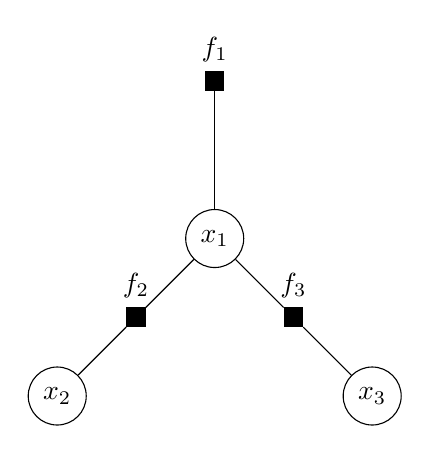
\begin{tikzpicture}[scale=1.0,transform shape]
   	\node[shape=circle,draw=black] (x1) at (0,0) {$x_1$};
    \node[shape=circle,draw=black] (x2) at (-2,-2) {$x_2$};
    \node[shape=circle,draw=black] (x3) at (2,-2) {$x_3$};
    \node[rectangle,draw=black, label = {$f_1$}, fill] (f1) at (0,2) {};
    \node[rectangle, fill, draw=black, label = {$f_2$}] (f2) at (-1,-1) {};
    \node[rectangle, fill, draw=black, label = {$f_3$}] (f3) at (1, -1) {} ;

    \path [-] (x1) edge node[left] {} (f1);
    \path [-] (x1) edge node[left] {} (f2);
    \path [-] (x1) edge node[left] {} (f3);
    \path [-] (f2) edge node[left] {} (x2);
    \path [-] (f3) edge node[left] {} (x3);
   
\end{tikzpicture}
\caption{Factor graph of $f$'s factorization into $f_1, f_2, f_3$ \newline Usually, variable nodes are drawn as circles whereas constraint nodes are drawn as rectangles to easily distinguish the types of nodes}

\end{figure}



\end{example}
% zu allgemein?
%
%A Constraint Satisfaction Problem (\textit{CSP}) consists of a set of variables $X = \{x_1, \ldots, x_n\}$, a set of domains $D = \{D_1, \ldots, D_n\}$ that specify which values each variable may take and a set of constraints $C = \{C_1, \ldots, C_m\}$ that must hold for the chosen values $x_i \in D_i$. \newline
%SAT can be written as CSP where each clause $C_j = {x_i, \ldots, x_k}$

%\newtheorem*{definition}{Definition}
\newpage
Factor graphs can also be used for describing constraint satisfaction problems. A factor corresponds to a constraint on its neighbour vertices, it evaluates to $1$ if the constraint is satisfied and to $0$ if not. For the global function $f$ - the product of all factors - to be $1$, every constraint has to be is satisfied. The special case of SAT problems is discussed in the following chapter.



\subsection{Factor Graph of a SAT Formula}
Any SAT formula over the variables $x_1, \ldots, x_n$ in CNF form can be interpreted as a function that factorizes to the formulas clauses. \newline
$x_1, \ldots, x_n$ are boolean variables which can be either $0$ or $1$. A SAT formula $\mathcal{F}$ is a conjunction / product of special constraints, the formula's \emph{clauses}. A clause is a disjunction of variables and their negations  $(x_i\lor \overline{x_j} \lor \ldots)$ and is satisfied if at least one variable $x_i$ that appears unnegated is set to $1$ or at least one $x_j$ that appears negated is set to $0$. \newline
In the factor graph of a formula each factor node $a$ represents the local function defined by a single clause. If the variable $x_i$ or its negation $\overline{x_i}$ appears in this clause the factor graph contains an edge between $a$ and the variable node $i$. 

In following descriptions the letters $a$ and $b$ always describe factor nodes, $i$ and $j$ are used for variable nodes. Also often no distinction is made between the nodes of the factor graph and the corresponding elements of the formula. Especially from here on variables are denoted as single letters $i, j$ whereas the value of a variable $i$ is written as $x_i \in \{0, 1\}$

In \cite{survprob} some additional notation is defined to simplify the description of the algorithms in section \ref{BPFS}: 
\newpage
\begin{definition} Let $a$ be a factor node and $i$ one of its variables.
\begin{itemize}
\item The value $J_i^a$ is $1$ if $i$ appears negated in $a$ and $-1$ if not
\item $V(a)$ is the set of all variables in $a$ \newline$V(i)$ is the set of all clauses containing $i$.  \newline Alternatively $V(a)$ and $V(i)$ are the neighbourhoods of $a$ and $i$ in the factor graph.
\item $V_+(a)$ is the set of variables that appear unnegated in $a$ \newline $V_-(a)$ is the set of $a$'s negated variables.
\item $V_a^u(i)$ is the set of $i$'s neighbours $b \neq a$ with $J_i^b \neq J_i^a$ \newline $V_a^s(i)$ is the set of neighbours $b \neq a$ with $J_i^b = J_i^a$\newline
The letters $u, b$ stand for \emph{(\textbf{u}n)\textbf{s}atisfied} meaning that if $i$ satisfies a clause $b \in V_a^s(i)$, it also satisfies $a$.
\end{itemize}
\end{definition}


\begin{example}
Let $$\mathcal{F} = \underbrace{(x_1 \lor x_2 \lor x_3)}_{a} \land \underbrace{(\overline{x_1} \lor x_2 \lor x_4) }_{b}\land \underbrace{(\overline{x_3} \lor x_4)}_{c} \land \underbrace{(\overline{x_1} \lor \overline{x_2})}_{d}$$

\begin{figure}[h]
\centering

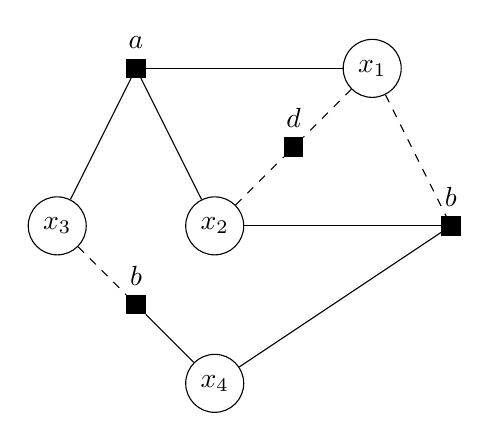
\begin{tikzpicture}[scale=1.0,transform shape]
   	\node[shape=circle,draw=black] (x1) at (3,0) {$x_1$};
    \node[shape=circle,draw=black] (x2) at (1,-2) {$x_2$};
    \node[shape=circle,draw=black] (x3) at (-1,-2) {$x_3$};
    \node[shape=circle,draw=black] (x4) at (1,-4) {$x_4$};
    
    \node[rectangle,draw=black, label = {$a$}, fill] (a) at (0,0) {};
     \node[rectangle,draw=black, label = {$d$}, fill] (d) at (2,-1) {};
     \node[rectangle,draw=black, label = {$b$}, fill] (b) at (4,-2) {};
     \node[rectangle,draw=black, label = {$b$}, fill] (c) at (0,-3) {};
     
 
    \path [-] (x1) edge node[left] {} (a);
    \path [-] (x2) edge node[left] {} (a);
    \path [-] (x3) edge node[left] {} (a);
    
    \path [dashed] (x1) edge node[left] {} (d);
    \path [dashed] (x2) edge node[left] {} (d);
    
    \path [-] (x2) edge node[left] {} (b);
    \path [dashed] (x1) edge node[left] {} (b);
    \path [-] (x4) edge node[left] {} (b);
    
    \path [-] (x4) edge node[left] {} (c);
    \path [dashed] (x3) edge node[left] {} (c);
\end{tikzpicture}
\caption{Factor graph of a $\mathcal{F}$}
\end{figure}

Again the circles are variable nodes, the rectangles are constraint nodes. If $x_i$ appears negated in the clause $a$ (if $J_a^i = 1$), the edge is drawn dashed. With the addition of dashed lines the factor graph completely describes the formula $\mathcal{F}$.

The variable sets of $b$ are for example $V(b) = \{1, 2, 4\}$, $V_+(b) = \{2, 4\}$, $ V_-(b) = \{1\}$.
The sets of $x_1$ are $V(1) = \{a, b, d\}$, $V_a^s(1) = \emptyset$, $V_a^u(1) = \{b, d\}$.

\end{example}
